\chapter{Theory}

\section{Quantum Linear System Problem (QLSP)}

The "Classical" Linear System Problem (LSP) states the following:
\\
Given an $N \times N$ matrix A, an $N-$dimensional vector $\Vec{b}$, and the equation
    \begin{equation*}
        A \Vec{x} = \Vec{b}
    \end{equation*}
solve for $\Vec{x} = (x_1, x_2,...,x_N)^T$. To date, the best algorithm for this task is called the Conjugate Transpose method first introduced by Hestenes and Stiefel in 1952 \cite{hestenes_methods_1952}. It has an asymptotic complexity of $O(N\cdot \sqrt{k})$, and thus complexity grows polynomially as the number of inputs increases. 

Analogously, the Quantum Linear System Problem (QLSP) states that given a Hermitian $N \times N$ matrix A, a unit vector $\Vec{b}$, and the equation
    \begin{equation*}
        A \Vec{x} = \Vec{b}
    \end{equation*}
prepare a quantum state that approximates
\begin{equation*}
    | x \rangle = \frac{\sum_{i=1}^N x_i | i \rangle}{\sqrt{(\sum_{i=1}^N | x_i |^2)}}
\end{equation*}
where $\Vec{x} = (x_1, x_2,...,x_N)^T$. Specifically, for a given precision $\epsilon > 0$, the approximate (mixed or pure) quantum state $\rho_x$ satisfies
\begin{equation*}
    \frac{1}{2}Tr|\rho_x - |x\rangle \langle x| | \leq \epsilon
\end{equation*}

\section{Quantum Algorithms for Solving Linear Systems}

A particular family of quantum algorithms leverage the powerful properties of subatomic particles, particularly superposition and entanglement, to approximate solutions to linear systems of equations. Arising from the wave-like behavior of particles, superposition refers to the ability of quantum state as a linear combination of other distinct quantum states. By distributing information stored among many qubits, each of which adopts many different states, superposition allows us to encode inputs with exponentially less resources, one of the most promising characteristics of quantum algorithms. In addition, when two particles get really close to each other their quantum states become interdependent; they become entangled. This characteristic allows quantum computers to massively distribute calculations among several entangled qubits. 

\subsection{HHL algorithm}

The Harrow-Hassidim-Lloyd (HHL) quantum algorithm, given a Hermitian matrix \textbf{A}, will compute the vector of unknowns $|x\rangle$ in the form $|x \rangle = \sum_{j=1}^N \beta_j \cdot \frac{1}{\lambda_j} |\textbf{u}_j \rangle$ where $\{ |\textbf{u}_j \rangle \}$ denotes the eigenvectors of A and $\{\lambda_j\}$ its eigenvalues. By encoding the amplitudes of the input information HHL only need polynomial logarithm of qubits with respect to the input size \cite{duan_survey_2020}. Then, HHL performs three important operations:
\begin{enumerate}
    \item Quantum Phase Estimation (QPE)
    \item Invert the eigenvalues
    \item Measurement
\end{enumerate}
QPE consists in estimating the phase of an eigenvalue of the unitary operator $U$ that we create by using the properties of Hermitian matrices. In Quantum Linear Solvers this phase is critical to efficiently compute, often by spectral decomposition, the input matrix's inverse and invert the eigenvalues in the eigenbasis of the given matrix during the second step. Finally, the algorithm measures the auxiliary qubit in the computational basis and if the outcome is 1, then the state of that qubit contains the solution. 

\begin{figure}[h!]
    \centering
    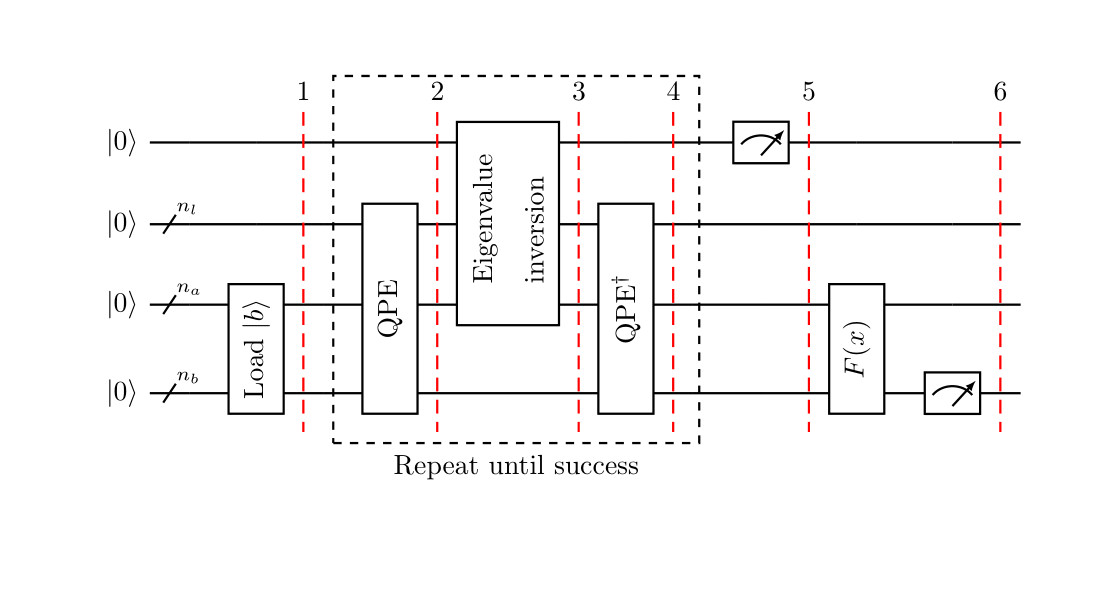
\includegraphics[scale=0.35]{images/hhlcircuit.png}
    \source{Source: \url{qiskit.org/textbook/ch-applications/hhl_tutorial.html}}
    \caption{HHL algorithm Circuit}
    \label{fig:my_label}
\end{figure}

The above graph depicts the circuit for HHL algorithm. After encoding the solution vector $|b \rangle$ as a linear combination of the input matrix A's eigenvectors, the algorithm undergoes an iterative process of inverting A's eigenvalues, by applying Quantum Phase Estimation with $U = e^{iAt}$, as well as computing A's inverse until the measurement (depicted in between lines 4 and 5) yields 1. Lastly, it returns the estimate $|\Tilde{x}\rangle \approx \sum_{j=1}^n \langle u_j|b \rangle / \lambda_j|u_j\rangle$ exponentially faster than the current best classical algorithm of conjugate gradient.

\section{A Hybrid Architecture to Solve the Riccati Equation}

The Matrix Riccati differential equation plays a key role in many applied fields including Control theory, theories of stabilization, transport theory, differential games and stochastic control.

I propose a hybrid algorithm to solve the Matrix Riccati differential equation given an initial condition. First, I show that some  Matrix Riccati equation can be turned to a linear system, given certain conditions are met, in which the matrix associated is Hermitian. Second, the mathematical findings are encoded in the classical component of the proposed algorithm. Third, I feed the Hermitian matrix output by step 1 to HHL on IBM's 4-qubit quantum computer, via IBM's quantum lab, and obtain the solution.

\subsection{Re-writing the Matrix Riccati equation}

Let R denote the following Matrix Riccati equation
\begin{equation}
\tag{R}
    Y' = Y\cdot A(t) \cdot Y + C(t)\cdot Y + Y\cdot B(t) + D(t)
\end{equation}
where $Y \in \mathbb{R}^{ n \times m}$, $D(t) \in \mathbb{R}^{ n \times m}$, $C(t) \in \mathbb{R}^{ n \times n}$, $B(t) \in \mathbb{R}^{m \times m}$ and $A(t) \in \mathbb{R}^{ m \times n}$.
The goal is, given an initial condition $Y(0)$, to obtain solutions $Y(t)$ for $t > 0$.

\begin{theorem}
Assuming $m = n$, if $B(t) = 0$ and if $A(t)$ is invertible, then R can be converted to the following second order matrix differential equation:
\begin{equation*}
    u'' - (ACA^{-1} + A'A^{-1})\cdot u' + AD \cdot u = 0
\end{equation*}

by using the change of variables $Y = - A^{-1} \cdot u' \cdot u^{-1}$, where $u$ is invertible. 
\end{theorem}

For conciseness, I will highlight the main steps of our proof, please refer to the Appendix for the full proof. 

\begin{theorem}
If $ACA^{-1} + A'A^{-1} = S$ where $S$ is a matrix with constant entries and diagonalizable, and $A \cdot D = -I$, then (R2) can be converted into the following equation:
    \begin{equation}
        \tag{R3}
        v'' - D_1 \cdot v' - v = 0
    \end{equation}
where $D_1$ is a diagonal matrix.
\end{theorem}


Please refer to the Appendix for the full proof. From (R3) we obtain the following linear system
\begin{equation}
    e^{-tM_{ii}} \cdot x_{ii} = w_{ii}
\end{equation}
where $M_{ii} = \big(\begin{smallmatrix}
      0 & 1\\
      1 & -\alpha_i
    \end{smallmatrix}\big)$, $\alpha_i$ denotes the entries in the diagonal of the matrix $D_1$, $w_{ii} = [v_{ii}(0), v'_{ii}(0)]^T$, where $v_{ij}$ are the entries of $v$ so $v = (v_{ij})$ and $1 \leq i,j \leq n$. 

Solving $e^{-tM_{ii}} \cdot x_{ii} = w_{ii}$ is equivalent of solving the system. 
\begin{equation*}
    H \cdot
    \begin{pmatrix}
        x_{11} \\
        x_{22} \\
        \vdots \\
        x_{nn}
    \end{pmatrix}
    = \Vec{w}
\end{equation*}
where 
\begin{equation*}
    H = \begin{pmatrix}
        e^{-tM_{11}} & 0 & 0 & ... & 0 \\
        0 & e^{-tM_{22}} & 0 & ... & 0 \\
        0 & 0 & e^{-tM_{33}} & ... & 0 \\
        0 & 0 & 0 & ... & e^{-tM_{nn}}
    \end{pmatrix}
    \text{and} \hspace{0.8mm} \Vec{w} = \begin{pmatrix}
        w_{11} \\
        w_{22} \\
        \vdots \\
        w_{nn}
    \end{pmatrix}
\end{equation*}

Note that $H$ is sparse and Hermitian for any $1 \leq i \leq n$. Thus, after normalizing the vector $\Vec{w}$, we can leverage the HHL quantum algorithm to gain an exponential advantage over current classical algorithms.
